\chapter{Results}
\label{cha:results}

In this chapter, the micro-location method proposed in this paper---mediation---will be discussed in greater detail.

\section{Architecture of the proposed solution}
\label{sec:architecture}

\Cref{fig:architecture} presents the overview of main components of the solution. The process happens in several steps, some of which are repeated at each run, some need to be done once only.

\begin{enumerate}
	\item First, the data about locations used for micro-location purposes, that is held in human heads, needs to be digitized into computer-readable maps in OpenGIS format.
	\item At approximately the same time, configuration file for the micro-located object/place has to be created. In it, there are changes of costs defined that add or subtract from the total cost of a generated question, based on various properties and types of objects included in the question1.
	\item The data contained in the maps is automatically transformed (parsed) into a format understood by the mediation engine\ldots
	
	\begin{figure}
		\centering
		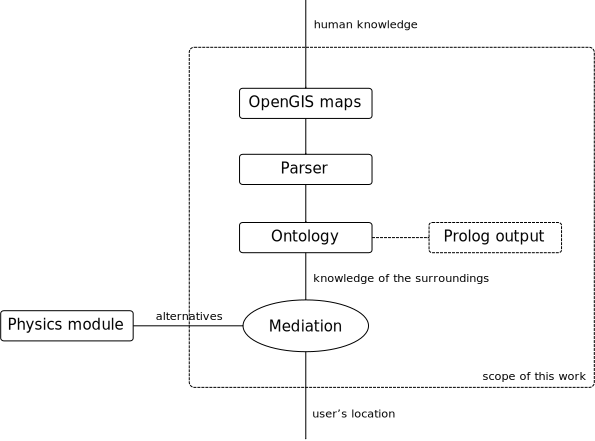
\includegraphics[width=\textwidth]{architecture}
		\caption{Architecture of the proposed solution (own work).}
		\label{fig:architecture}
	\end{figure}
	
	\item \ldots{}namely the ontology.
	\item An optional step that can be taken, is to export the ontology as a Prolog source code, that can be later used in some further research, as Prolog is particularly excelling at Artificial Intelligence prototyping.
	\item An external physics-based module needs to provide the mediation module with some alternative pre-guessed locations for the latter to choose from.
	\item Immediately after the alternatives are provided, the mediation starts. Using the knowledge of the surroundings (from the ontology) and rules concerning costs (from the configuration), several questions are presented to the user. Answers enable successful inference of their location.
\end{enumerate}

\section{OpenGIS maps}

Because of the fact that for all examples evaluated in this work (\cref{cha:evaluation}), parsing of their corresponding maps took less than a second, the parsing step is performed at each start time of the mediation engine. Thanks to that, the data is kept in its rawest form possible, i.e. just the maps. That makes it also easier for the administrative user, as no manual intermediate preparatory step is needed, when creating the data.

OpenGIS maps created for the sake of examples/evaluation in this work were made using the OpenJUMP\footnote{\url{https://web.archive.org/web/20150804110932/http://www.openjump.org/} (visited on 08/04/2015).} editor. This program creates a structure of files and directories corresponding to \emph{layers} defined by the user. A layer consists of several objects added to it at precisely defined position. The concept of layers doesn't play any role in mediation and thus they are only added as a convenience for the user creating the maps. Any object added to a layer---apart from its position in space---is also characterized by a map of properties in form of key--value pairs. In \cref{fig:opengis-props-map} such properties can be seen in the editor, while \cref{lst:opengis-props-onto} has these properties translated into Prolog source code. The properties are what has the greatest significance in the mediation process, as they enable discerning of objects; one of the properties takes a role of defining a class of an object (in ontological sense) and can be chosen at each parsing step.

\begin{figure}
	\centering
	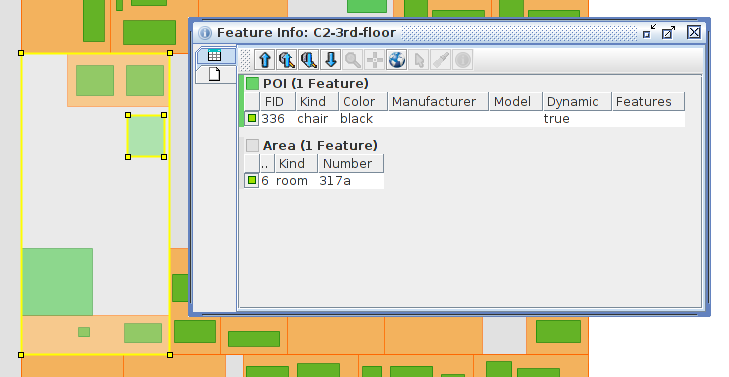
\includegraphics[width=\textwidth]{opengis-props-map}
	\caption{Properties of a ``chair'' object in OpenJUMP map editor.}
	\label{fig:opengis-props-map}
\end{figure}

\begin{lstlisting}[language=Prolog,caption={Ontology exported to Prolog source code for room ``317a'' containing the ``chair'' from \cref{fig:opengis-props-map} at line 10.},numbers=left,columns=flexible,basicstyle=\ttfamily,label=lst:opengis-props-onto]
room{number: "317a"} has [
  fridge{color: "white"} exists,
  desk{color: "light brown"} has [
    microwave{color: "gray"} exists,
    kettle{color: "white"} exists
  ],
  wardrobe{color: "light brown"} has [
    display{color: "gray"} exists * 2
  ],
  chair{color: "black", dynamic: "true"} exists,
  wall{color: "white"} has [ door{} exists * 2 ]
].
\end{lstlisting}

\section{Ontology}

As seen in \cref{lst:opengis-props-onto}, optional export of the ontology to a Prolog format is supported, e.g. for further research. Also, dumping it like that makes debugging significantly easier, as the ontology that is used directly for mediation has no textual representation.

\todo{finish}

\section{Configuration}

\todo{finish}

\section{Physics-based module for providing alternative possible user locations}
\label{sec:physics-module}

To get a few alternative location (an input to the mediation process, ``where the user might be''), an external physics-based module is used. The one used currently is the subject of work of Bobek and Grodzki among others, and more about it can be read in \cite{bobek2015indoor, Koeping2015indoor}. Therein, details of mathematical models used are presented.

The basic idea is to use two sources of data. If inferred locations occupy more than one room, mediation is triggered. The sources are:

\begin{itemize}
	\item dead-reckoning (pedometer) using data from various motion sensors of a device (accelerometer, gyroscope) and
	\item strength of signals received from iBeacon-compatible transmitters placed in rooms.
\end{itemize}

Dead-reckoning (also known as ``inertial measurements'') works by changing the model's idea of user's location, incrementally adding and subtracting small changes to it (steps in this case). Amounts of these changes are inferred based on data coming from motion sensors of a devices using a mathematical model. As Köping et al. state in \cite{Koeping2015indoor}, ``We model the indoor localization problem as a recursive density estimation problem, which can be estimated by employing the Bayesian framework, namely particle filters.''

The idea for using beacons in the module is to make an assessment about distances to nearby transmitters based on signal strength and RSSI (one case of the law of inverse squares, see \cref{eq:inverse-sq} and \cref{sec:existing-uloc}). Arguably, this could potentially be seen as somewhat of a misuse of the iBeacon technology. Manufacturers generally speak of \emph{three} recognizable levels of ``interaction'' with the beacon (based on signal strength): \begin{itemize}
 	\item receiver being in very close proximity to the transmitter,
 	\item receiver being in the same room,
 	\item no interaction at all.
 \end{itemize}
 
Matyasik et al. claim that the RSSI-to-distance-based approach works, however, \emph{only under laboratory conditions} \cite{Matyasik:iBeacon, Matyasik:iBeacon:slides}. As iBeacons use extremely low energy to transmit the signal, even a single person walking across the room while taking the measurement---or even someone playing with the smartphone during the measurement---can influence it so negatively, that any information inferred about the distance to the signal's source cannot be reliably trusted.

\section{The process of mediation}

The shortcomings of iBeacons and dead-reckoning (\cref{sec:physics-module}) encourage the use of some additional data source. In this work, mediation is proposed.

\todo{entropy}

\todo{how is intelligibility achieved?}

\todo{alternatives can be provided in attr=val form; we can ask with high granularity}

\todo{finish}

\section{User Experience}
\label{sec:user-experience}

\todo{finish}
